\section{Teoria MCSCF}
\subsection{Introduzione}

Il successo della teoria HF \`e dovuto alla sua relativa efficienza
applicato a sistemi closed shell. Grazie a tale teoria, \`e possibile
ottenere un set spinorbitalico (orbitali canonici) da
utilizzare in successive trattazioni.
Si pu\`o ricavare che, al fine di minimizzare l'energia di un 
monodeterminante $\Phi = \detsl{\psi_1 \ldots \psi_n} $, deve essere, per il
teorema di Brillouin
\beq
\braket{\Phi}{\ham}{\Phi_i^a} = 0 
\eeq
ovvero non ci deve essere interazione tra lo stato $\Phi$ e una sua
singola eccitazione. Questo conduce, grazie alle regole di Slater,
alla relazione tra spinorbitali
\beq
\braket{\psia}{\fock}{\psii} = 0
\eeq

Di conseguenza, $\fock\psii$ \`e uno spinorbitale totalmente
ortogonale allo spazio degli spinorbitali virtuali, e come tale
appartiene allo spazio degli occupati. Da ci\`o si ottiene
\beq
\fock\psii = \sumonen{j}\psij\epsilon_{ji}
\eeq

Esister\`a quindi un particolare set spinorbitalico che, oltre a
soddisfare il teorema di Brillouin (e quindi rendere minima l'energia
HF), diagonalizza anche la matrice $\epsilon_{ji}$, il set di orbitali
canonici. 

I valori diagonali di tale matrice prendono il nome di \textbf{energie
orbitaliche}, e per il teorema di Koopmans (Cfr. \cite{tp-1-1933-104})
\beq
E_+^i-E_0 = -\epsilon_i
\eeq
rappresentano approssimativamente l'energia di ionizzazione in gioco
durante la rimozione di un elettrone dall'orbitale \textit{i}-esimo (Cfr.
\cite{jce-75-11-1998-1494})

Tale trattazione \`e tuttavia insoddisfacente per molecole con una geometria
non prossima a quella di equilibrio, durante l'analisi di
legami in via di dissociazione o per lo studio di stati eccitati. 
La principale approssimazione deriva dal supporre che la configurazione
della molecola in studio sia data esclusivamente dal monodeterminante di
Slater considerato. Tale approssimazione si ripercuote in una errata
valutazione dell'energia. L'errore commesso va sotto il nome di
\textbf{energia di correlazione}, e la sua stima \`e centrale in tutte le
trattazioni post Hartree-Fock.

Per questa ragione, una prima via alla valutazione del contributo
correlativo \`e descrivere la molecola come una sovrapposizione
di pi\`u configurazioni elettroniche (approccio multiconfigurazionale).
Durante la rottura di legami, ma anche in molti altri casi, specie quando
stati quasi degeneri entrano in gioco, una descrizione monodeterminantale
non \`e sufficiente a garantire che la descrizione HF sia una
approssimazione sufficiente dello stato di interesse.

\subsection{Un caso semplice: l'idrogeno}
\label{subsec:idrogeno}
La molecola di idrogeno \`e il caso accademico pi\`u noto. Gli orbitali
molecolari sono comunemente scritti come combinazione lineare di orbitali
atomici (Linear Combination of Atomic Orbitals, LCAO) dei due atomi, per cui:
\beq
\varphi_1=N_1 \left(1s_a + 1s_b \right)
\eeq

Dal momento che tale orbitale spaziale \`e doppiamente occupato,
il determinante di Slater sar\`a ovviamente
\beq
\Phi_1 = \varphi_1(1) \varphi_1(2) \frac{\alpha \beta - \beta \alpha}{\sqrt{2}}
\eeq
Utilizzando tale descrizione elettronica per la distanza di equilibrio, i risultati
ottenuti sono in ragionevole accordo con il dato sperimentale.

Svolgendo il prodotto della funzione $ \Phi_1 $
\beqa
\Phi_1 &=& N_1^2 \left( 1s_a (1) + 1s_b (1)\right) \left( 1s_a (2) + 1s_b (2)\right) \mathcal{S}_0 (s_1,s_2) \nonumber \\
&=& N_1^2 \left[ \left( 1s_a (1) 1s_a (2) + 1s_b (1) 1s_b (2) \right) \right. \nonumber \\
& & + \left. \left( 1s_a (1) 1s_b (2) +  1s_b (1) 1s_a (2) \right) \right] \mathcal{S}_0 (s_1,s_2)
\eeqa
dove con $\mathcal{S}_0 (s_1, s_2)$ si indica la funzione di spin
$\frac{\alpha \beta - \beta \alpha}{\sqrt{2}}$, \`e possibile riconoscere una
componente ionica (che vede la coppia elettronica in possesso di un solo
atomo) e una componente covalente (che vede gli elettroni equamente
distribuiti su entrambi gli atomi).  Tale trattazione assegna alle
componenti lo stesso peso, a qualsiasi
distanza interatomica.
Come conseguenza, l'energia SCF ottenuta da tale trattazione \`e
totalmente errata a grandi distanze internucleari, dove soltanto la
componente covalente sopravvive.
\begin{center}
\vspace{0.3cm}
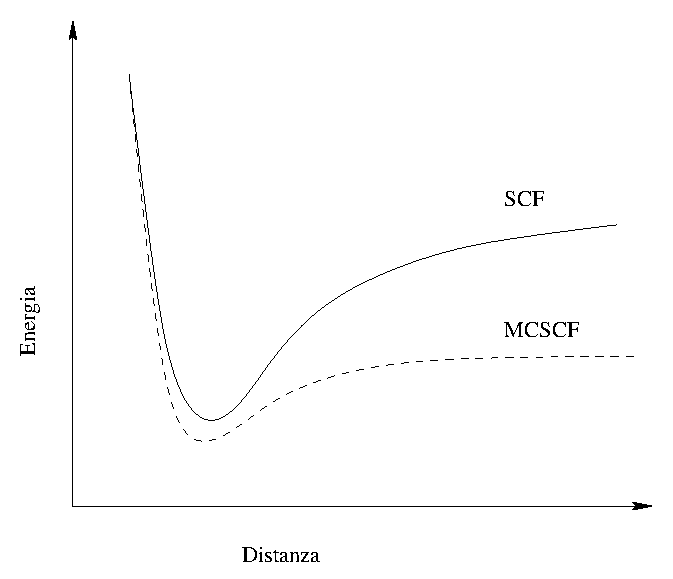
\includegraphics{immagini/SCF-MCSCF.eps} 
\vspace{0.3cm}
\end{center}

Possiamo migliorare la trattazione ipotizzando che la funzione sia descritta
da una combinazione lineare di stati, aggiungendo l'antilegame
\beq
\varphi_2=N_2 \left( 1s_a - 1s_b \right)
\eeq
e scrivendo quindi la funzione d'onda MC
\beq
\Psi_{MC} = c_1 \Phi_1 + c_2 \Phi_2
\eeq
dove
\beq
\Phi_2 = \varphi_2(1) \varphi_2(2) \frac{\alpha \beta - \beta \alpha}{\sqrt{2}}
\eeq
Questa funzione presenta una combinazione, variabile con la distanza, tra le
componenti covalente e ionica, e mostra il corretto comportamento asintotico.

In questo semplice caso, due elettroni vengono distribuiti
su 2 orbitali. Purtroppo anche in molecole semplici, come ossigeno e
azoto, il numero di orbitali e di elettroni con cui trattare risulta
abbastanza elevato. Questo si traduce in una eccessiva complessit\`a computazionale,
nel caso in cui lo scopo fosse una trattazione completa delle possibili distribuzioni
elettroniche. Questa modalit\`a di risoluzione, denominata Full-CI, prende in
considerazione tutte le possibili distribuzioni degli elettroni negli orbitali,
ed \`e la tecnica che fornisce il miglior risultato, per una data
base spinorbitalica. Sebbene ideale, questa strategia \`e raramente 
percorribile proprio a causa dell'eccessivo peso computazionale anche su molecole
piccole.

Al fine di semplificare, e di aprire la possibilit\`a di trattare molecole
di maggiori dimensioni senza pregiudicare il risultato ottenuto, si \`e
optato per includere all'interno della funzione d'onda solo quei determinanti
che si ritengono necessari alla descrizione della molecola. Si parla in questo caso di funzioni
di tipo Multi Reference. Lo schema di selezione dei determinanti da considerare
delinea il metodo multireference scelto.
Uno dei pi\`u noti metodi di selezione, il CAS (Complete Active Space) prevede la
suddivisione dello spazio orbitalico in 3 insiemi: 
\begin{itemize}
\item orbitali virtuali, sempre vuoti
\item orbitali attivi, riempiti in tutti i modi possibili (0, 1, 2
elettroni)
\item orbitali di core, completamente riempiti.
\end{itemize}

Il metodo si basa sulla semplificazione di considerare tutte le possibili
disposizioni degli elettroni solo internamente allo spazio degli
orbitali attivi. Questo riduce la complessit\`a computazionale, e al
tempo stesso tenta di introdurre i maggiori contributi correlativi rispetto
alla semplice funzione HF.

\subsection{Metodo MCSCF e seconda quantizzazione}

Si abbia un set spinorbitalico $ \left\{ \psi_1 \psi_2
\ldots \psi_{n} \right\}$. Usando tali spinorbitali, \`e possibile costruire
un generico determinante di Slater per 3 elettroni
\beq
\Phi = \detsl{\psi_1 \psi_2 \psi_5}
\eeq
Definiamo ora gli operatori di creazione e distruzione, la cui azione
rispettivamente \`e l'aggiunta o la rimozione di uno spinorbitale ad un
determinante, secondo le seguenti regole: per il distruttore, indicato con
la simbologia $\destr{i}$, se lo spinorbitale bersaglio $i$ \`e presente
\beqas
\destr{i}
\detsl{\psi_1,\psi_2,\ldots,\psi_{i-1},\psi_i,\psi_{i+1},\ldots,\psi_{2n}} & = &
(-1)^{p_i} \detsl{\psi_1,\psi_2,\ldots,\psi_{i-1},\psi_{i+1},\ldots,\psi_{2n}}
\eeqas
dove $p_i$ \`e il numero di trasposizioni necessarie a portare lo spinorbitale
bersaglio $i$ in prima posizione nel determinante.
Nel caso lo spinorbitale sia assente, il risultato \`e zero.

Per l'operatore di creazione, indicato con la simbologia $\constr{i}$, se
lo spinorbitale bersaglio $i$ \`e assente
\beqas
\constr{i} \detsl{\psi_1 \psi_2 \ldots } & = &
\detsl{\psi_i \psi_1 \psi_{2} \ldots }
\eeqas
in caso contrario (spinorbitale gi\`a presente), il risultato \`e zero.

\`E utile ricordare le regole di anticommutazione per gli operatori di
creazione e distruzione
\beqas
\constr{i}\constr{j}+\constr{j}\constr{i} = 0 \\
\destr{i}\destr{j}+\destr{j}\destr{i} = 0 \\
\constr{i}\destr{j}+\destr{j}\constr{i} = \delta_{ij}
\eeqas
come anche l'operatore di eccitazione/diseccitazione $\constr{i}\destr{j}$ che
sostituisce in un determinante lo spinorbitale $\psi_j$ con $\psi_i$
\beq
\constr{i}\destr{j} \detsl{\psi_1 \psi_2 \ldots \psi_j \ldots \psi_n} =
\detsl{\psi_1 \psi_2 \ldots \psi_i \ldots \psi_n}
\eeq
Possiamo anche definire un operatore spin traced
\beq
E_{ij} = \left( \constr{i\alpha}\destr{j\alpha} +
\constr{i\beta}\destr{j\beta} \right)
\eeq
che si riferisce agli orbitali molecolari spaziali,
indipendentemente dal fattore di spin.

Valgono le propriet\`a
\begin{itemize}
\item $ \left[ E_{ij}, E_{kl} \right] = E_{il}\delta_{jk} -
E_{kj}\delta_{il} $
\item $ E^{+}_{ij} = E_{ji} $
\end{itemize}

\subsection{Operatori in seconda quantizzazione}

Mediante il formalismo della seconda quantizzazione, \`e possibile
scrivere gli operatori quantistici secondo un differente approccio.
Un generico operatore monoelettronico pu\`o essere espanso sulla base di
operatori di creazione e distruzione
$$
\hat{F} = \sumidx{i,j} F_{ij} \constr{i}\destr{j}
$$
dove $F_{ij}$ \`e l'elemento di matrice
$$
F_{ij} = \int \! \psii^{*}(x)\hat{F}(x)\psij(x) \: dx
$$

Utilizzando gli operatori $E_{ij}$ si pu\`o ottenere
$$
\hat{F} = \sumidx{i,j} F_{ij}E_{ij}
$$
dove gli indici $i$ e $j$ ora sono indici orbitalici puramente spaziali
e l'integrale $F_{ij}$ \`e ora definito su una base spaziale.

Analogamente possiamo definire un operatore bielettronico
$$
\hat{G} = \sumidx{i,j,k,l} g_{ijkl} \constr{i}\constr{j}\destr{l}\destr{k}
$$
dove $g_{ijkl}$ \`e l'integrale
$$
g_{ijkl} = \int \! \! \! \! \int \! \psii^*(x_1) \psij^*(x_2) \hat{G}(x_1,x_2) \psik(x_1)
\psil(x_2) \, dx_1 dx_2
$$

Sommando sullo spin, dopo alcune manipolazioni, \`e possibile ottenere il
risultato
$$
\hat{G} = \half \sumidx{i,j,k,l} g_{ijkl} \left( E_{ik} E_{jl} -
\delta_{jk} E_{il} \right)
$$
dove, al solito, gli indici corrono ora su orbitali puramente spaziali.

In conclusione, l'hamiltoniano in seconda quantizzazione \`e scrivibile
come
$$
\ham = \sumidx{i,j} h_{ij} E_{ij} + \half \sumidx{i,j,k,l} g_{ijkl}
\left( E_{ik} E_{jl} - \delta_{kj} E_{il} \right)
$$

\subsection{Trasformazione di base}

Al fine di rendere minima l'energia, occorre effettuare una trasformazione 
sia sui coefficienti della nostra funzione MC, sia sulla base spinorbitalica 
su cui costruiamo i vari determinanti.

Le trasformazioni della base spinorbitalica possono essere viste come rotazioni in uno spazio
orbitalico, attuate da un operatore opportuno. Dal momento che la
rotazione non cambia la dimensionalit\`a della base, il risultato
appartiene ancora allo spazio delle funzioni spinorbitaliche di
partenza, e come tale \`e esprimibile come una opportuna combinazione
lineare dei vettori della base iniziale
$$
\mbox{\boldmath $\varphi$}^{\prime} = \mbox{\boldmath $\varphi$}\mathbf{U}
$$
dove {\boldmath $\varphi$} \`e un vettore riga contenente gli spinorbitali di
partenza, {\boldmath $\varphi^{\prime}$} \`e la base ottenuta dalla trasformazione e
$\mathbf{U}$ \`e una matrice unitaria che attua la trasformazione stessa.

Dal momento che viene attuata una trasformazione sulla base, anche gli
operatori di creazione e distruzione andranno incontro ad una trasformazione.
\`E possibile esprimere tale trasformazione attraverso
la relazione
\beq
\constr{i}{}^\prime = e^{\left(-\hat{T}\right)} \constr{i}
e^{\left(\hat{T}\right)}
\eeq
e analogamente per il distruttore. L'operatore $\hat{T}$ \`e
antihermitiano, che pu\`o essere espanso, come operatore
monoelettronico, nella forma
\beq
\hat{T}=\sumidx{i,j}T_{ij}\constr{i}\destr{j}
\eeq
dove i coefficienti $T_{ij}$ definiscono una matrice $\mathbf{T}$ antihermitiana (ovvero
\mbox{$\mathbf{T}^{+} = - \mathbf{T}$})

Si dimostra che \`e possibile trasformare un generico determinante di 
Slater applicando l'operatore $e^{-\hat{T}}$:
\beqas
% 
\ket{m'}= a{'}_i^+ a{'}_j^+ \ldots\vacuum & = &
e^{\left(-\hat{T}\right)} \constr{i} e^{\left(\hat{T}\right)}
e^{\left(-\hat{T}\right)}\constr{j} e^{\left(\hat{T}\right)}\ldots\vacuum
\\
% 
& = & e^{\left(-\hat{T}\right)}\constr{i} \constr{j}\ldots\vacuum \\
%
& = & e^{\left(-\hat{T}\right)}\ket{m}
\eeqas

Dal momento che la trasformazione attuata sugli orbitali
avviene esclusivamente sulla parte spaziale, la matrice di
trasformazione $\mathbf{T}$ \`e partizionata in 4 sottomatrici
\beq
\mathbf{T} = \left(
\begin{array}{cc}
\mathbf{T}_{\alpha\alpha} & \mathbf{T}_{\alpha\beta} \\
\mathbf{T}_{\beta\alpha} & \mathbf{T}_{\beta\beta}
\end{array}
\right)
\eeq

Se, in seguito al cambiamento di base, non si effettua mescolamento tra
orbitali con occupazione $\alpha$ e orbitali con occupazione $\beta$, i
termini delle sottomatrici fuori  diagonale $\mathbf{T}_{\alpha\beta}$ e
$\mathbf{T}_{\beta\alpha}$ sono nulli. Inoltre, dato che le trasformazioni
sono le stesse per lo stesso set spaziale, $\mathbf{T}_{\alpha\alpha} = \mathbf{T}_{\beta\beta}$.
Con queste relazioni, l'operatore $\hat{T}$ risulta
\beqa
%
\hat{T} & = & \sumidx{i,j} \left( T_{ij}^{\alpha\alpha} \constr{i\alpha}
\destr{j\alpha} 
+ T_{ij}^{\alpha\beta} \constr{i\alpha} \destr{j\beta}
+ T_{ij}^{\beta\alpha} \constr{i\beta} \destr{j\alpha}
+ T_{ij}^{\beta\beta} \constr{i\beta} \destr{j\beta} \right) \nonumber \\
%
& = & \sumidx{i,j} T_{ij} \left( \constr{i\alpha} \destr{j\alpha} +
\constr{i\beta} \destr{j\beta} \right) \nonumber \\
%
& = & \sumidx{i,j} T_{ij}E_{ij}
\eeqa
supponendo la matrice antihermitiana $\mathbf{T}$ reale, si avr\`a $T_{ij} = -T_{ji}$ e
quindi
\beq
\hat{T} = \sumidx{i>j} T_{ij}\left(E_{ij} - E_{ji}\right) 
= \sumidx{i>j} T_{ij} E_{ij}^-
\eeq
dove con l'ultimo termine si esprime una scrittura abbreviata.

\subsection{Metodo risolutivo Newton-Raphson}

L'ottimizzazione di una funzione d'onda multiconfigurazionale prevede
di modificare sia gli orbitali base, sia i coefficienti della combinazione
lineare di determinanti.
Uno dei metodi di risoluzione \`e conosciuto come metodo Newton-Raphson, o
metodo NR: l'assunto di partenza \`e considerare l'energia del sistema $E$ come
funzione di un vettore di parametri $\mathbf{p}$, e quindi espandere
tale dipendenza in serie di Taylor attorno un punto $\mathbf{p}_0$.
Si avr\`a
\beq
E(\mathbf{p}) = E(\mathbf{p}_0) + \sumidx{i} \left( \frac{\partial E}{\partial
p_i}\right)_{\mathbf{p}_0} p_i + \half \sumidx{i,j} p_i \left( \frac{\partial^2 E}{\partial
p_i \partial p_j} \right)_{\mathbf{p}_0} p_j + \ldots
\eeq
che in notazione matriciale diventa
\beq
E(\mathbf{p}) = E(\mathbf{p}_0) + \mathbf{g}^+\mathbf{p} + \half
\mathbf{p}^+\mathbf{H}\mathbf{p} + \ldots
\eeq
dove $\mathbf{g}$ \`e un vettore detto \textit{gradiente energia} e
$\mathbf{H}$ \`e la \textit{matrice Hessiana} dell'energia.

Affinch\`e si abbia un minimo, la derivata prima dell'energia rispetto 
a tutti i parametri deve essere zero, ovvero il vettore gradiente nullo.
Per risolvere tale problema, si ricorre ad una procedura iterativa 
che prevede la risoluzione dell'equazione lineare
\beq
\mathbf{g} + \mathbf{Hp} = \mathbf{0} 
\eeq

\subsection{Ottimizzazione dei parametri e degli orbitali}

L'ottimizzazione dei parametri e degli orbitali passa attraverso l'uso
di operatori unitari. \`E gi\`a stato presentato l'operatore $\hat{T}$, 
che attua una rotazione dello spazio orbitalico. Analogamente,
\`e possibile definire un operatore unitario $\hat{S}$ che attua una
trasformazione sui coefficienti della combinazione lineare.

L'energia dello stato MC $\ket{0}$ sar\`a quindi definita
\beq
E(\mathbf{T},\mathbf{S}) =
\braket{0}{e^{\left(-\hat{S}\right)}e^{\left(-\hat{T}\right)}\ham e^{\left(\hat{T}\right)}e^{\left(\hat{S}\right)}}{0}
\eeq
Espandendo con l'identit\`a di Glauber\footnote{Ricordiamo l'identit\`a di Glauber 
\beqas
e^{\hat{A}}\hat{B}e^{-\hat{A}} & = & \hat{B} + \left[ \hat{A} , \hat{B}
\right] + \frac{1}{2!} \left[ \hat{A} , \left[ \hat{A} , \hat{B} \right]
\right] + \frac{1}{3!} \left[ \hat{A} , \left[ \hat{A} , \left[ \hat{A} ,
\hat{B} \right] \right] \right] + \ldots
\eeqas
} tale espressione, si ottiene
\beqas
E(\mathbf{T},\mathbf{S}) & = & \left\langle 0 \left| \ham + \left[\ham,\hat{T}\right] 
+ \left[\ham,\hat{S}\right] 
+ \half \left[ \left[ \ham,\hat{T}\right],\hat{T}\right] \right. \right. \\
& & \left. \left. + \half \left[ \left[ \ham,\hat{S}\right],\hat{S}\right]
+ \left[ \left[ \ham,\hat{T}\right],\hat{S}\right]
+ \ldots \right| 0 \right\rangle
\eeqas

Il primo termine rende conto dell'energia di ordine zero
$E(\mathbf{0},\mathbf{0})$. Il successivo pu\`o essere sviluppato
\beqas
\braket{0}{\left[\ham,\hat{T}\right]}{0} & = & \sumidx{i,j} T_{ij}
\braket{0}{\left[\ham,E_{ij}\right]}{0} \\
%
& = & \sumidx{i,j} T_{ij} g_{ij}^{(o)}
\eeqas
dove abbiamo posto
\beq
g_{ij}^{(o)} = \braket{0}{\left[\ham,E_{ij}\right]}{0}
\eeq
Il simbolo $(o)$ indica che la trasformazione \`e a carico degli
orbitali.

Ora \`e necessario ottenere l'operatore per la trasformazione a
carico dei coefficienti. Sia innanzitutto definito l'operatore di rotazione
sui coefficienti $\hat{S}$ come
\beq
\hat{S} = \sumidx{K\neq0} S_{K0} \left(\ket{K}\bra{0} - \ket{0}\bra{K}
\right)
\eeq
dove $\ket{K}$ sono generici stati, espansi sulla medesima base
spinorbitalica, tali da essere ortogonali tra loro.

Svolgendo opportunamente il commutatore
\beq
\braket{0}{\left[\ham,\hat{S}\right]}{0} =
\sumidx{K\neq0}S_{K0} \left( \braket{0}{\ham}{K} + \braket{K}{\ham}{0}
\right)
\eeq
che con autofunzioni reali, per hermitianit\`a, conduce ad ottenere
\beq
g_K^{(c)} = 2 \braket{0}{\ham}{K}
\eeq
vettore che esprime la derivata prima effettuata su una
variazione dei coefficienti della funzione MC.

\`E possibile procedere in modo analogo ricavando la matrice
\textit{hessiana}, responsabile della trasformazione al secondo ordine.
Si otterranno 3 contributi: un contributo (oo) di trasformazione sugli 
orbitali, un contributo (cc) di trasformazione sui coefficienti e 
un contributo (co) = (oc) di variazione accoppiata orbitali-coefficienti.

Ora, riprendendo e riadattando
\beqas
\mathbf{g} + \mathbf{Hp} = \mathbf{0} \\
\mathbf{Hp} = - \mathbf{g}
\eeqas
si pu\`o scrivere, in definitiva
\beq
\left(
\begin{array}{cc}
\half \mathbf{H}^{(cc)} & \half \mathbf{H}^{(co)} \\
\left( \half \mathbf{H}^{(co)} \right)^+ & \half \mathbf{H}^{(oo)} \\
\end{array}
\right) 
\left(
\begin{array}{c}
\mathbf{S} \\
\mathbf{T} \\
\end{array}
\right) = -
\left(
\begin{array}{c}
\half \mathbf{g}^{c} \\
\half \mathbf{g}^{o} \\
\end{array}
\right)
\eeq

Il metodo Newton-Raphson prevede la risoluzione iterativa di questo
sistema o analoghi (al fine di semplificare il metodo computazionale),
tuttavia richiede che il vettore di guess per il processo iterativo
sia sufficientemente vicino al minimo locale verso cui si vuole convergere. In
caso contrario, il metodo pu\`o convergere molto lentamente o addirittura
divergere. Sono quindi necessarie procedure per identificare una zona
di minimo, in cui definire in modo approssimativo un vettore di guess.

\subsection{Metodo Super-CI}
Un metodo alternativo all'approccio Newton-Raphson \`e il cosiddetto
metodo Super-CI.
Tale metodo prevede di annullare l'interazione con gli stati
monoeccitati mediante una procedura iterativa.
Per risolvere tale problema, si costruisce una funzione Super-CI come
$$
\ket{SCI} = \ket{0} + \sumidx{p>q}t_{pq}E_{pq}^-\ket{0}
$$
dove $E_{pq}^- = E_{pq} - E_{qp}$.
La funzione d'onda SCI \`e una combinazione di uno stato base MC e delle
sue eccitazioni. Il metodo prevede di ottenere la convergenza quando
$\braket{0}{\ham}{E_{pq}^- 0} = 0$ come affermato dal teorema di Brillouin,
esteso a casi multireference (Cfr. \cite{ijqc-2-1968-307}).

Una particolarit\`a del metodo risiede nella non ortogonalit\`a delle
singole eccitazioni
\beqas
S_{pq,rs} &=& \integral{E_{pq}^-0}{E_{rs}^-0} \\
&=& \braket{0}{E_{qp}^-E_{rs}^-}{0} \\
& \neq & \delta_{pq,rs}
\eeqas
le funzioni non sono nemmeno normalizzate ($S_{pq,pq} \neq 1$).

Gli elementi di matrice dell'hamiltoniano hanno la forma
\beqas
\braket{0}{\ham}{pq} &=& \braket{0}{\ham E_{pq}^-}{0} = w_{pq} \\
\braket{pq}{\ham}{rs} &=& \braket{0}{E_{qp}^-\ham E_{rs}^-}{0} = d_{pq,rs}
\eeqas
L'equazione secolare da risolvere sar\`a quindi
$$
\left(
\begin{array}{cc}
E_{MC} & \mathbf{w}^+ \\
\mathbf{w} & \mathbf{d}
\end{array} \right)
\left(
\begin{array}{c}
1 \\
\mathbf{t} \\
\end{array}
\right)
= E_{SCI}
\left(
\begin{array}{cc}
1 & \mathbf{0} \\
\mathbf{0} & \mathbf{S}
\end{array}
\right)
\left(
\begin{array}{c}
1 \\
\mathbf{t} \\
\end{array}
\right)
$$
che pu\`o anche essere riscritta come
$$
\left(
\begin{array}{cc}
0 & \mathbf{w}^+ \\
\mathbf{w} & \mathbf{d}-E_{MC}\mathbf{S}
\end{array} \right)
\left(
\begin{array}{c}
1 \\
\mathbf{t} \\
\end{array}
\right)
= \left( E_{SCI} - E_{MC} \right)
\left(
\begin{array}{cc}
1 & \mathbf{0} \\
\mathbf{0} & \mathbf{S}
\end{array}
\right)
\left(
\begin{array}{c}
1 \\
\mathbf{t} \\
\end{array}
\right)
$$

Il metodo Super-CI converge sempre in un minimo locale, al contrario del
metodo Newton-Raphson che pu\`o convergere anche in punti di sella.

